\documentclass{beamer}
%
% Choose how your presentation looks.
%
% For more themes, color themes and font themes, see:
% http://deic.uab.es/~iblanes/beamer_gallery/index_by_theme.html
%
\mode<presentation>
{
  \usetheme{default}      % or try Darmstadt, Madrid, Warsaw, ...
  \usecolortheme{default} % or try albatross, beaver, crane, ...
  \usefonttheme{default}  % or try serif, structurebold, ...
  \setbeamertemplate{navigation symbols}{}
  \setbeamertemplate{caption}[numbered]
} 

\usepackage[english]{babel}
\usepackage[utf8]{inputenc}
\usepackage[T1]{fontenc}

\title[Your Short Title]{Algebraic Filtering of Surfaces from 3D Medical Images with Julia}
\author{Alberto Paoluzzi, Miroslav Jirik}
\institute{Roma Tre University, Charles University}
\date{CAD 2020}

\begin{document}

\begin{frame}
  \titlepage
\end{frame}

% Uncomment these lines for an automatically generated outline.
%\begin{frame}{Outline}
%  \tableofcontents
%\end{frame}



\section{Introduction}

\begin{frame}
\begin{columns}
\end{columns}
\begin{figure}
    \centering
    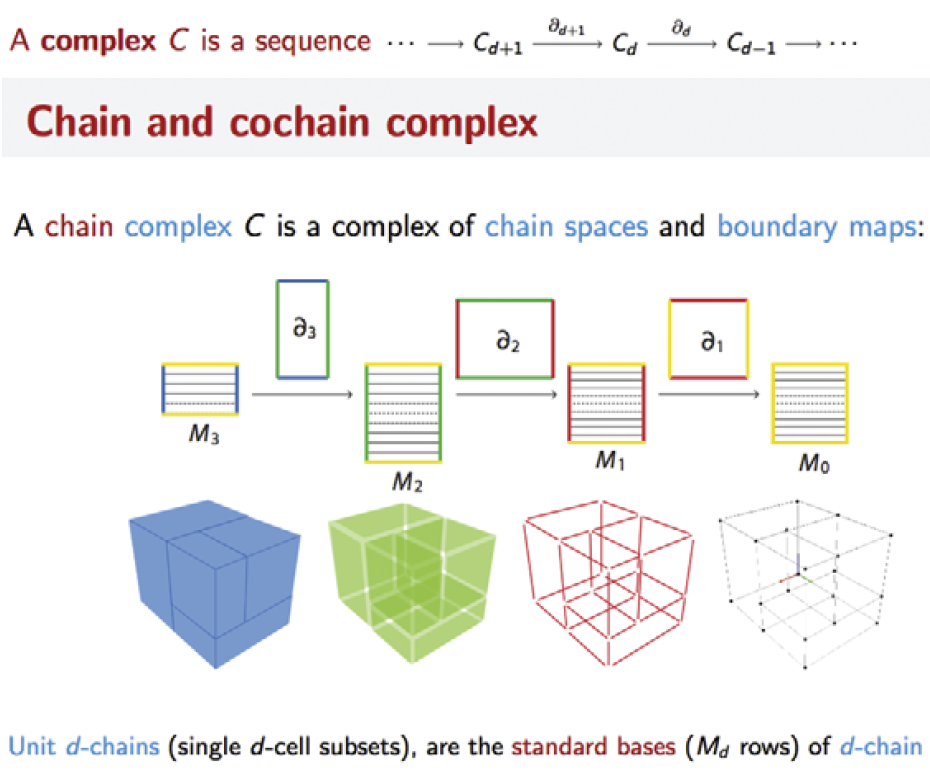
\includegraphics[width=0.95\textwidth]{figs/L02-chain-complex.png}
    % \caption{Caption}
    % \label{fig:my_label}
\end{figure}
    
\end{frame}




\begin{frame}
\begin{figure}
    \centering
    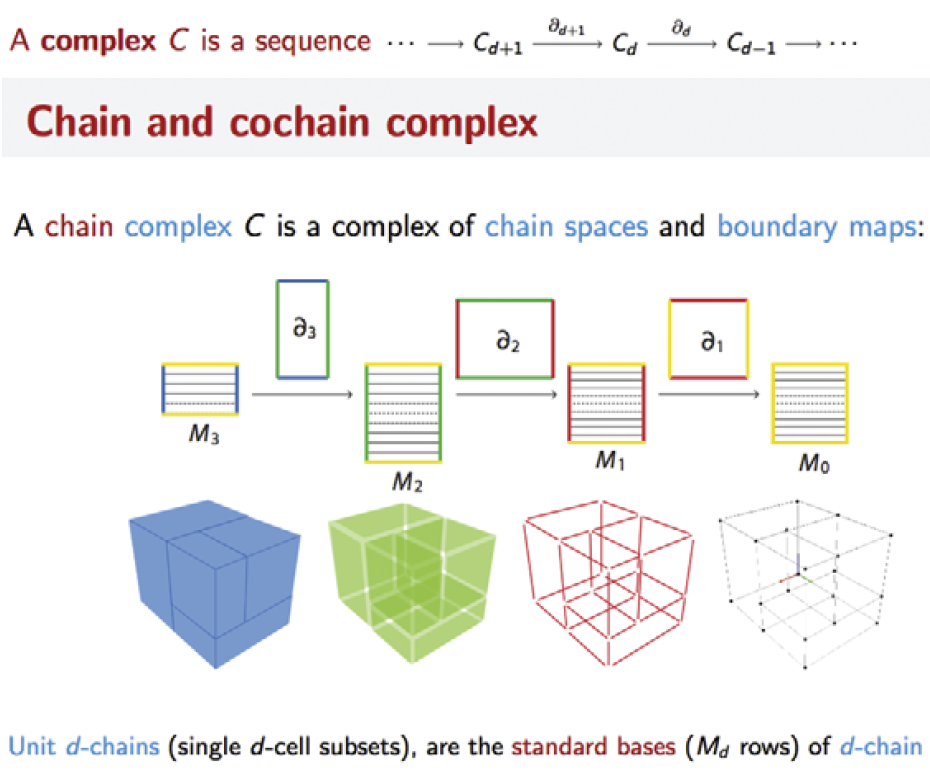
\includegraphics[width=0.95\textwidth]{figs/L02-chain-complex.png}
    % \caption{Caption}
    % \label{fig:my_label}
\end{figure}
    
\end{frame}


\begin{frame}
\begin{figure}
    \centering
    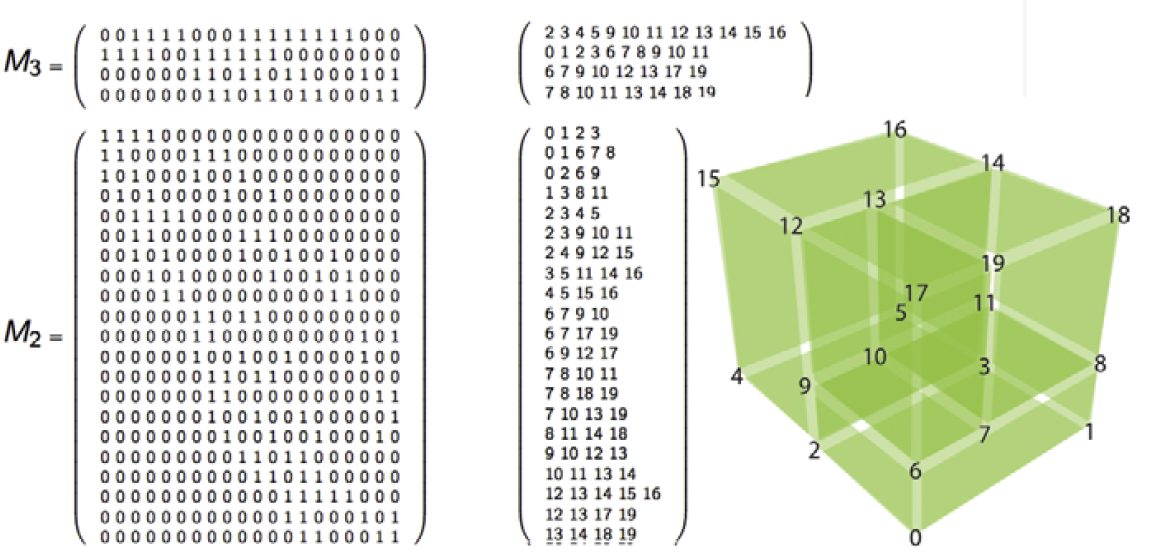
\includegraphics[width=\textwidth]{figs/L02-characteristic-matrices.png}
    % \caption{Caption}
    % \label{fig:my_label}
\end{figure}
\end{frame}


\begin{frame}{Lar-surf}
\begin{figure}
    \centering
            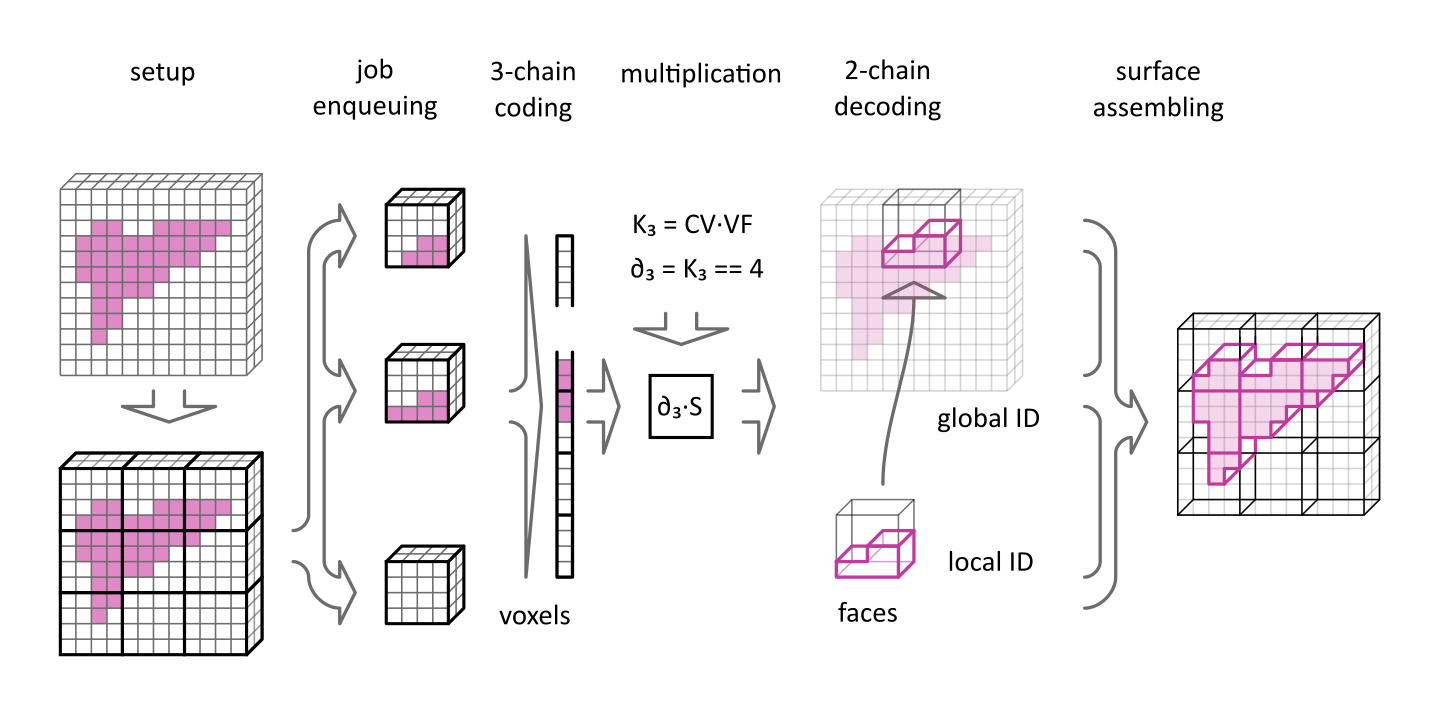
\includegraphics[width=\textwidth]{figs/schema_horizontal.png}
    \caption{LAR surface extraction scheme}
\end{figure}
    
\end{frame}

\begin{frame}{Surface extraction with LAR}
\begin{figure}
    \centering
            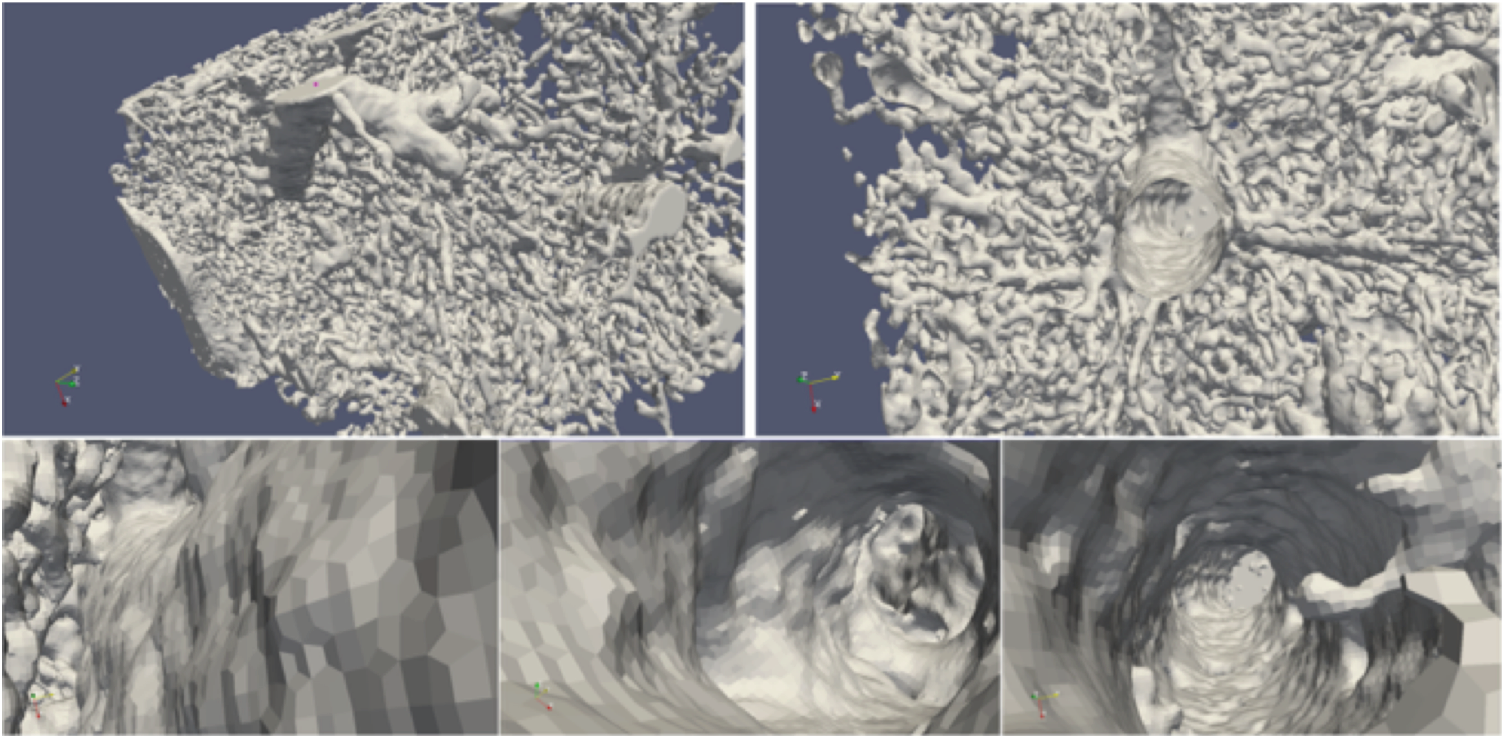
\includegraphics[width=\textwidth]{figs/paoluzzi_dicarlo_furiani_jirik_2016.png}
    \caption{Liver microstructure\cite{Paoluzzi2016}}
\end{figure}
    
\end{frame}


\begin{frame}{Surface extraction with LAR}
\begin{figure}
    \centering
            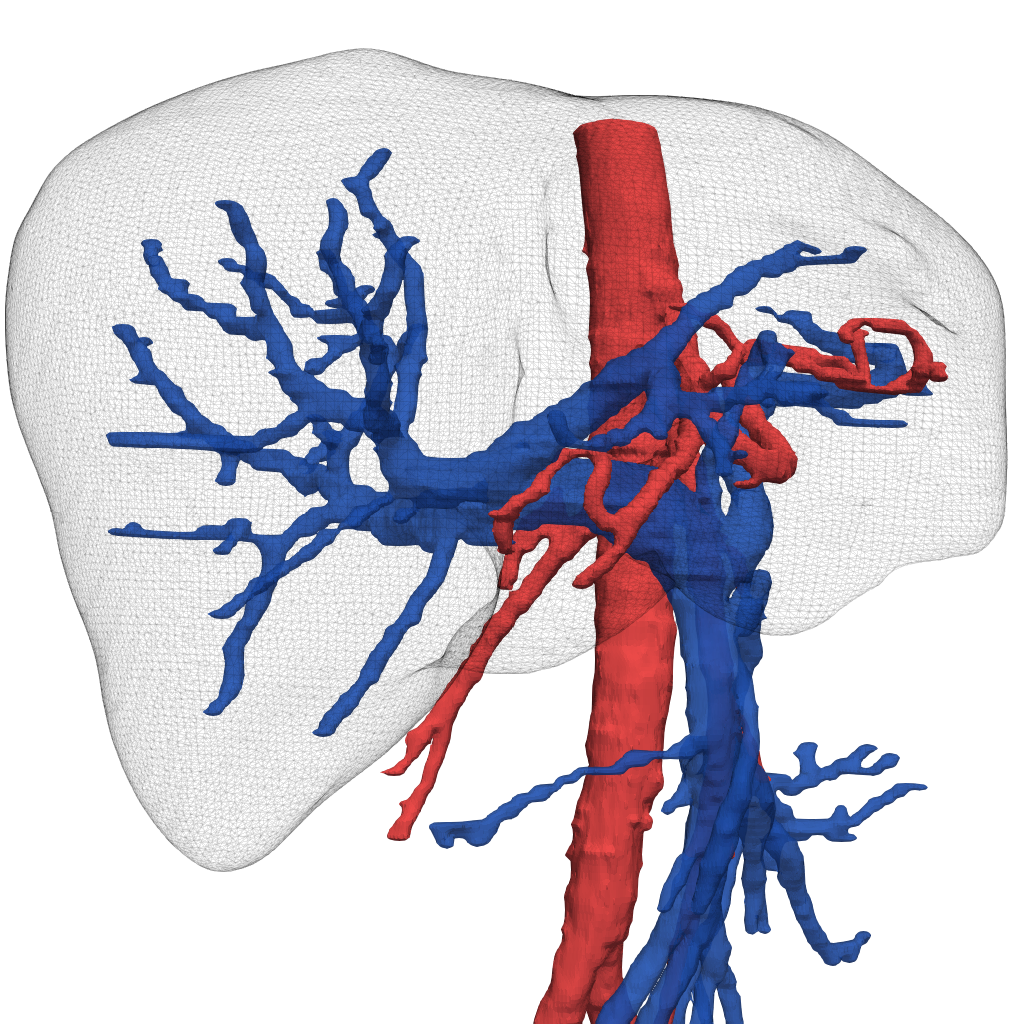
\includegraphics[width=0.6\textwidth]{figs/ircad01_liver_tricolore_01.png}
\end{figure}
    
\end{frame}



\begin{frame}{Introduction}

\begin{itemize}
  \item Your introduction goes here!
  \item Use \texttt{itemize} to organize your main points.
\end{itemize}

\vskip 1cm

\begin{block}{Examples}
Some examples of commonly used commands and features are included, to help you get started.
\end{block}

\end{frame}

\section{Some \LaTeX{} Examples}

\subsection{Tables and Figures}

\begin{frame}{Tables and Figures}

\begin{itemize}
\item Use \texttt{tabular} for basic tables --- see Table~\ref{tab:widgets}, for example.
\item You can upload a figure (JPEG, PNG or PDF) using the files menu. 
\item To include it in your document, use the \texttt{includegraphics} command (see the comment below in the source code).
\end{itemize}

% Commands to include a figure:
%\begin{figure}
%\includegraphics[width=\textwidth]{your-figure's-file-name}
%\caption{\label{fig:your-figure}Caption goes here.}
%\end{figure}

\begin{table}
\centering
\begin{tabular}{l|r}
Item & Quantity \\\hline
Widgets & 42 \\
Gadgets & 13
\end{tabular}
\caption{\label{tab:widgets}An example table.}
\end{table}

\end{frame}

\subsection{Mathematics}

\begin{frame}{Readable Mathematics}

Let $X_1, X_2, \ldots, X_n$ be a sequence of independent and identically distributed random variables with $\text{E}[X_i] = \mu$ and $\text{Var}[X_i] = \sigma^2 < \infty$, and let
\[ S_n = \frac{X_1 + X_2 + \cdots + X_n}{n}
      = \frac{1}{n}\sum_{i}^{n} X_i \]
denote their mean. Then as $n$ approaches infinity, the random variables $\sqrt{n}(S_n - \mu)$ converge in distribution to a normal $\mathcal{N}(0, \sigma^2)$.

\end{frame}

\begin{frame}[t,allowframebreaks]
\frametitle{References}
\bibliographystyle{alpha}
\bibliography{references.bib}
\end{frame}

\end{document}
